
%\section{How to Use this Template}

%The template details the sections that can be used in a manuscript. Note that the order and names of article sections may differ from the requirements of the journal (e.g., the positioning of the Materials and Methods section). Please check the instructions on the authors' page of the journal to verify the correct order and names. For any questions, please contact the editorial office of the journal or support@mdpi.com. For LaTeX-related questions please contact latex@mdpi.com.
%The order of the section titles is: Introduction, Materials and Methods, Results, Discussion, Conclusions for these journals: aerospace,algorithms,antibodies,antioxidants,atmosphere,axioms,biomedicines,carbon,crystals,designs,diagnostics,environments,fermentation,fluids,forests,fractalfract,informatics,information,inventions,jfmk,jrfm,lubricants,neonatalscreening,neuroglia,particles,pharmaceutics,polymers,processes,technologies,viruses,vision

\section{Introduction}

%The introduction should briefly place the study in a broad context and highlight why it is important. It should define the purpose of the work and its significance. The current state of the research field should be reviewed carefully and key publications cited. Please highlight controversial and diverging hypotheses when necessary. Finally, briefly mention the main aim of the work and highlight the principal conclusions. As far as possible, please keep the introduction comprehensible to scientists outside your particular field of research.  %Please use the command \citep{} for the following MDPI journals, which use author--date citation: Administrative Sciences, Arts, Econometrics, Economies, Genealogy, Histories, Humanities, IJFS, Journal of Intelligence, Journalism and Media, JRFM, Languages, Laws, Religions, Risks, Social Sciences.
 
%%%%%%%%%%%%%%%%%%%%%%%%%%%%%%%%%%%%%%%%%%
\section{Materials and Methods}

%Materials and Methods should be described with sufficient details to allow others to replicate and build on published results. Please note that publication of your manuscript implicates that you must make all materials, data, computer code, and protocols associated with the publication available to readers. Please disclose at the submission stage any restrictions on the availability of materials or information. New methods and protocols should be described in detail while well-established methods can be briefly described and appropriately cited.

%Research manuscripts reporting large datasets that are deposited in a publicly avail-able database should specify where the data have been deposited and provide the relevant accession numbers. If the accession numbers have not yet been obtained at the time of submission, please state that they will be provided during review. They must be provided prior to publication.

%Interventionary studies involving animals or humans, and other studies require ethical approval must list the authority that provided approval and the corresponding ethical approval code.
%\begin{quote}
%This is an example of a quote.
%\end{quote}

\subsection{Cycle Component Modeling}

\subsubsection{Heat Exchangers}
\subsubsection{Turbines}
\subsubsection{Compressors}
\subsubsection{Concentrating Solar Power Cycle}


\subsection{Cycle Models}








%%%%%%%%%%%%%%%%%%%%%%%%%%%%%%%%%%%%%%%%%%%%%%%%%%%%%%%%%%%%%%%%%%%%%%%%%%%%%%%%%%
\section{Results}

%This section may be divided by subheadings. It should provide a concise and precise description of the experimental results, their interpretation as well as the experimental conclusions that can be drawn.

There are various cycles that have been modeled to test their advantages and disadvantages. These various models cycles two different categories: non-charging and charging. The non-charging category will decide the configuration of the cycle with a focus on generating electricity. This includes the number of turbines, recuperators, and where heat is put into the system by the CSP and LFR. The charging category tests different locations of where heat is drawn from the LFR to be stored in the CSP's TES for later use.

\subsection{Non-Charging Cycle Configurations}%===================================

The cycles presented are generalized in order to draw a more direct comparison between cycles. These general parameters include isentropic efficiencies, heat exchanger approach temperatures, pressures, heat input, and pump constants. These values are summarized in Table \ref{cycle-constants}.


\begin{specialtable}[H] 
    \caption{Constant cycle parameters with definition, variable and set value. \label{cycle-constants}}
    \begin{tabular}{lcc}
    \toprule
    \textbf{Parameter} & \textbf{Variable}	& \textbf{Design Point Value}\\
    \midrule
    \textit{Efficiencies}\\
    Main Compressor & $\eta_{MC}$		& 0.91 (-)\\
    Re-Compressor & $\eta_{RC}$		& 0.89 (-)\\
    Turbine & $\eta_{T}$		& 0.90 (-)\\
    Pump & $\eta_{P}$      & 0.90 (-)\\
    \midrule
    \textit{Approach Temperatures}\\
    Low Temperature Recuperator & $\delta_{LTR}$		& 10 (K)\\
    High Temperature Recuperator & $\delta_{HTR}$		& 10 (K)\\
    Concentrating Solar Power Heat Exchanger & $\delta_{CSPHX}$	& 10 (K)\\
    \midrule
    \textit{Pressures}\\
    Pressure Ratio & $PR$ & 3.27 (-)\\
    High Side Pressure & $P_{2A}$ & 2.88e7 (Pa)\\
    \midrule
    \textit{Heat Into System}\\
    Lead-Fast Reactor Heat Transfer & $\dot{Q}_{LFRHX}$ & 9.5e8 (W)\\
    Concentrating Solar Power Heat Transfer & $\dot{Q}_{CSP}$ & 7.5e8 (W)\\
    \midrule
    \textit{Temperature}\\
    Main Compressor Inlet & $T_{1A}$ & 313.2 (K)\\
    Lead-Fast Reactor Low Temperature & $T_{4}$,$T_{1C}$,$T_{5A}$,$T_{4C}$ & 673.2 (K)\\
    \midrule
    \textit{Pumps}\\
    Pressure Rise Across Pump & $\Delta_{P}$ & 3.726e6 (Pa)\\
    Pump Low Side Pressure & $P_{S5-B}$ & 3.0e6 (Pa)\\ 
    \bottomrule
    \end{tabular}
\end{specialtable}

The values displayed in Table \ref{cycle-constants} are representative of LFR and CSP design while being consistent with design parameters given by our industry partner, Westinghouse Electric Corporation.


\subsubsection{Two-Cycle Configuration: C-LFR-ON and C-CSP-ON} %--------------------------------------------------------

The first cycle that will be tested has independent sCO$_{2}$ loops bridged by the CSP. This cycle has two Brayton Cycles: a LFR cycle and a CSP cycle. These two cycles individually operate when the focus of plant operation is primarily electricity generation.

The LFR cycle for this two-cycle configuration is labeled as C-LFR-ON and the cycle diagram is illustrated in Figure \ref{c-lfr-on}.

\end{paracol}
\begin{figure}[H] 
    \widefigure
    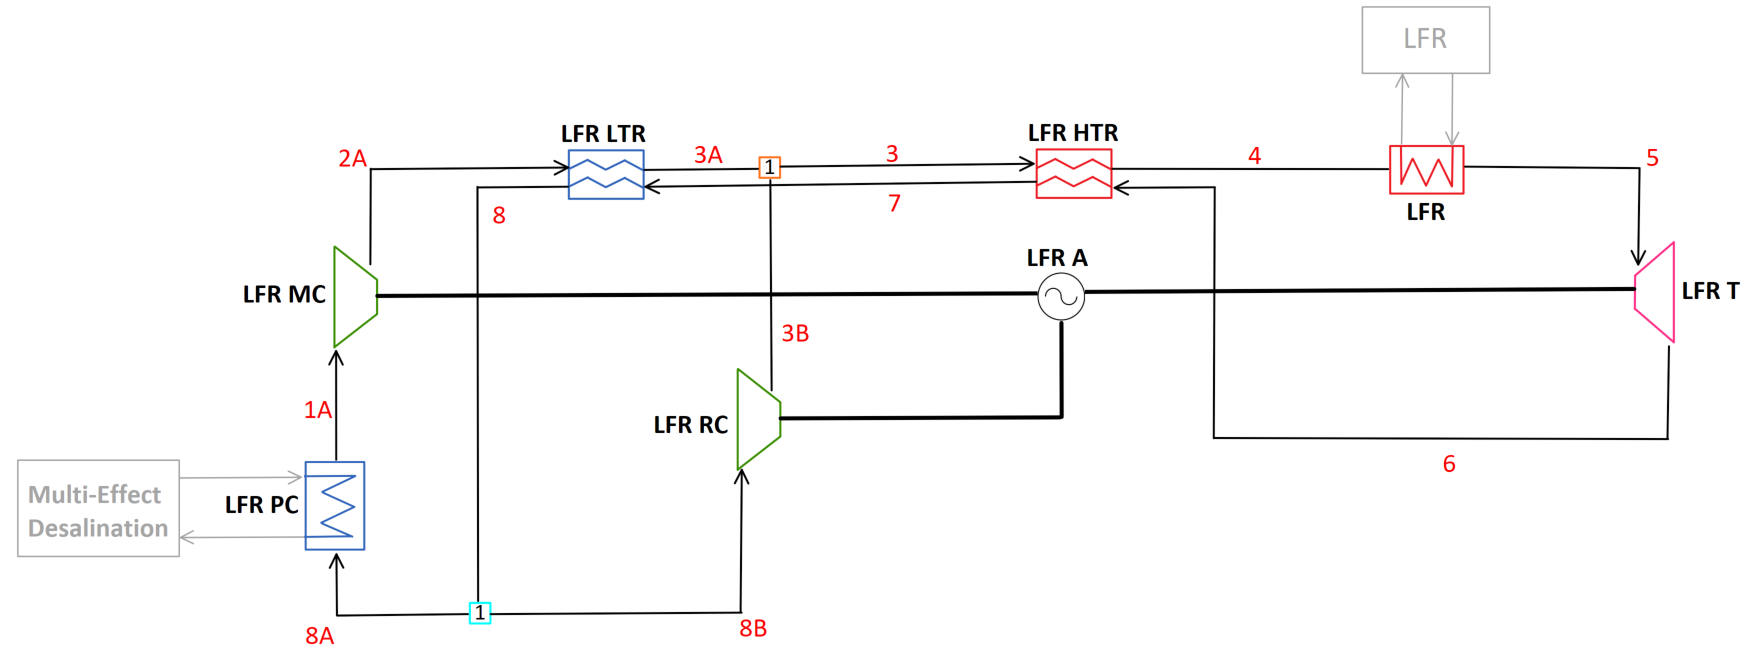
\includegraphics[width=\linewidth]{Definitions/c-lfr-on.pdf}
    \caption{Diagram for C-LFR-ON with focus on electricity generation\label{c-lfr-on}}
\end{figure}
\begin{paracol}{2}
\linenumbers
\switchcolumn

Modeling the C-LFR-ON cycle in EES yeilded the results in Table \ref{tab-c-lfr-on}. Two seperate sensitivity studies were completed on the LFR inlet temperature. The unconstrained (\textit{U}) values were from parametric studies on mass flow to the main compressor while maximizing cycle efficiency. The constrained (\textit{C}) values were calculated by setting the LFR inlet temperature to the design value of 673.2 K.

\begin{specialtable}[H] 
    \caption{Calculated system parameters for non-charging C-LFR-ON cycle configuration with constrained (\textit{C}) and unconstrained (\textit{U}) Lead-Fast Reactor low-end temperature.\label{tab-c-lfr-on}}
    \begin{tabular}{lccc}
    \toprule
    \textbf{Definition} & \textbf{Variable} & \textit{U} & \textit{C}\\
    \midrule
    LFR Inlet Temperature (K)	&	$T_{4}$	&	Data	&	Data	\\
    Cycle Efficiency (\%)	&	$\eta_{cycle}$	&	Data	&	Data	\\
    Alternator Power (W)	&	$\dot{W}_{A}$	&	Data	&	Data	\\
    PC Heat Transfer	&	$\dot{Q}_{PC}$	&	Data	&	Data	\\
    MC Power (W)	&	$\dot{W}_{MC}$	&	Data	&	Data	\\
    RC Power (W)	&	$\dot{W}_{RC}$	&	Data	&	Data	\\
    Turbine Power (W)	&	$\dot{W}_{T}$	&	Data	&	Data	\\
    MC Mass Flow Fraction (-)	&	$y_{1}$	&	Data	&	Data	\\
    LTR UA Value (W/K)	&	$UA_{LTR}$	&	Data	&	Data	\\
    LTR Capacitance Ratio (-)	&	$CR_{LTR}$	&	Data	&	Data	\\
    LTR Heat Transfer Rate (W)	&	$\dot{Q}_{LTR}$	&	Data	&	Data	\\
    LTR Effectiveness (-)	&	$\varepsilon_{LTR}$	&	Data	&	Data	\\
    HTR UA Value (W/K)	&	$UA_{HTR}$	&	Data	&	Data	\\
    HTR Capacitance Ratio (-)	&	$CR_{HTR}$	&	Data	&	Data	\\
    HTR Heat Transfer Rate (W)	&	$\dot{Q}_{HTR}$	&	Data	&	Data	\\
    HTR Effectiveness (-)	&	$\varepsilon_{HTR}$	&	Data	&	Data	\\
    \bottomrule
    \end{tabular}\\
\end{specialtable}

\textbf{Discussion of Results}

The CSP cycle for this two-cycle configuration is labeled C-CSP-ON and the cycle diagram is shown in Figure \ref{c-csp-on}. The CSP is shown in this diagram with the necessary pumps, TES tanks, and salt heat exchanger.

\end{paracol}
\begin{figure}[H] 
    \widefigure
    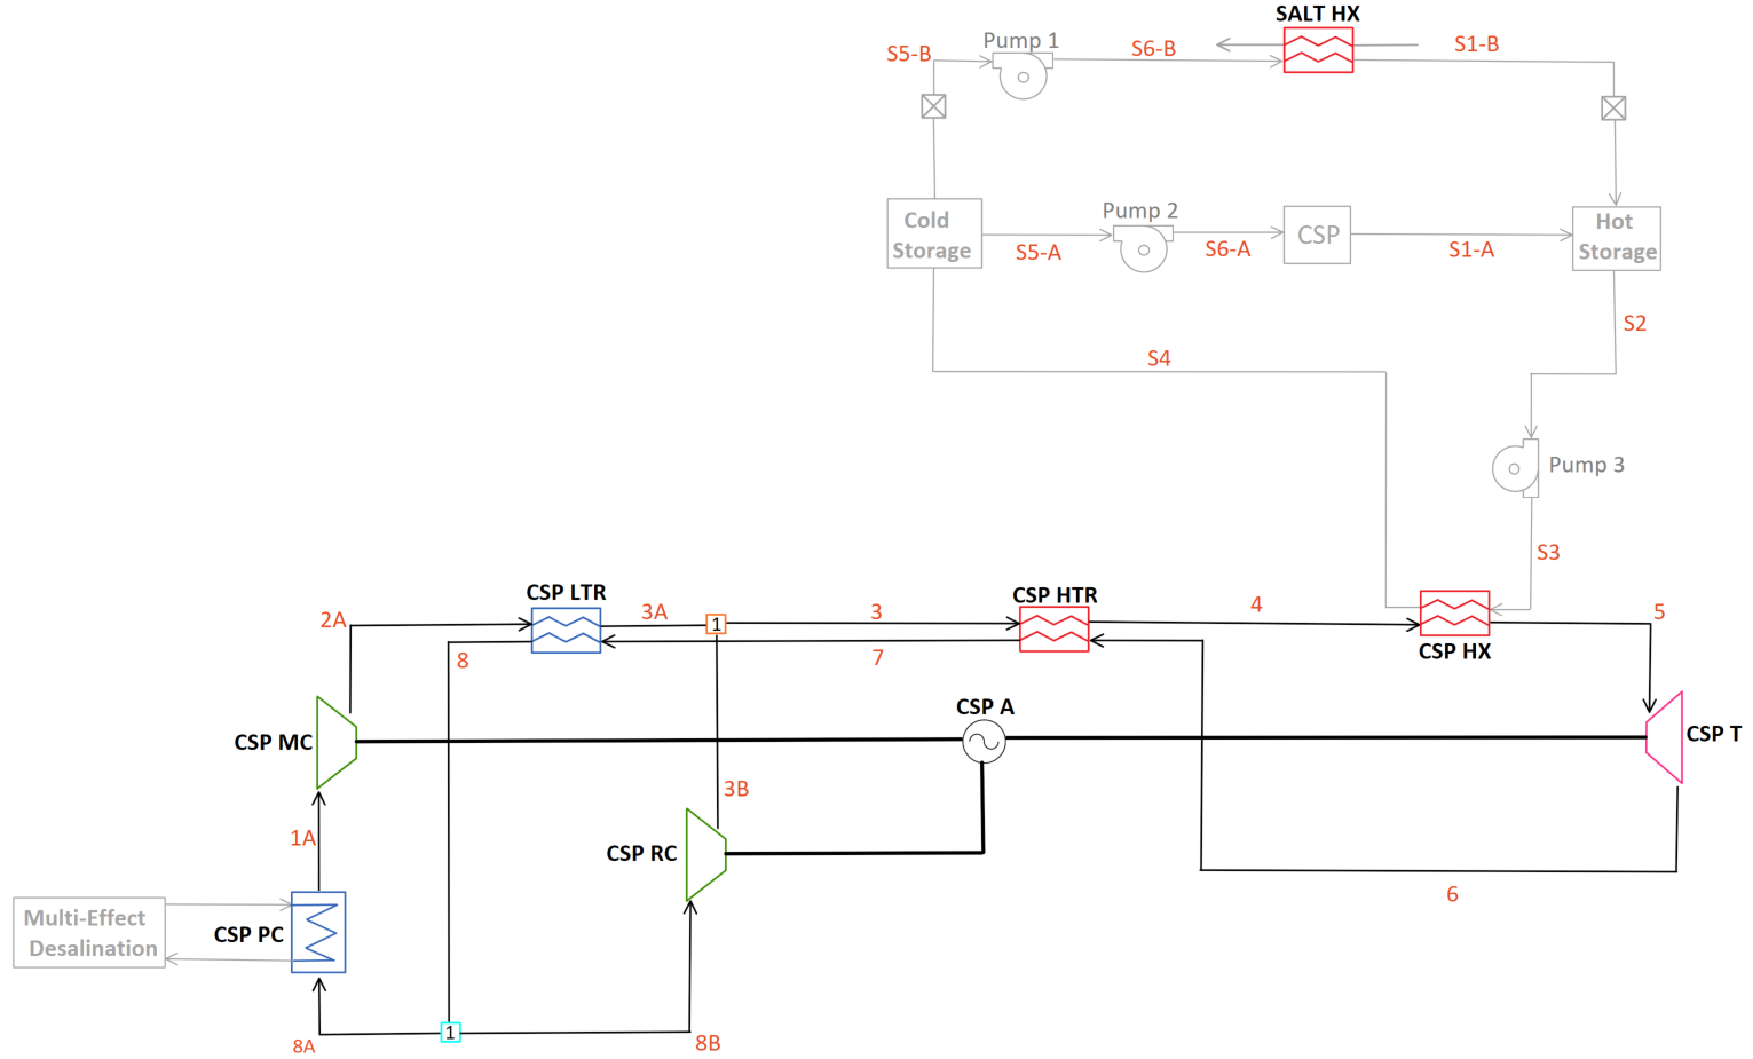
\includegraphics[width=\linewidth]{Definitions/c-csp-on.pdf}
    \caption{Diagram for C-CSP-ON with focus on electricity generation\label{c-csp-on}}
\end{figure}
\begin{paracol}{2}
\linenumbers
\switchcolumn

 C-CSP-ON is not directly impacted by constrained or unconstrained LFR low temperatures because it is an independent cycle while focused on electricity generation. Instead a sensitivity study was done on the temperature of the cold TES. Two temperatures were tested, 663.2 K and 713.2 K, to observe the impacts on cycle efficiency. The EES model outputs for C-CSP-ON are listed in Table \ref{tab-c-csp-on}.

\begin{specialtable}[H] 
    \caption{Calculated system parameters for non-charging C-CSP-ON cycle configuration with varied TES cold temperature. \label{tab-c-csp-on}}
    \begin{tabular}{lccc}
    \toprule
    \textbf{Definition} & \textbf{Variable} &  &\\
    \midrule
    Cold TES Temperature (K)	&	$T_{CS}$	&	Data	&	Data	\\
    Cycle Efficiency (\%)	&	$\eta_{cycle}$	&	Data	&	Data	\\
    Alternator Power (W)	&	$\dot{W}_{A}$	&	Data	&	Data	\\
    PC Heat Transfer	&	$\dot{Q}_{PC}$	&	Data	&	Data	\\
    MC Power (W)	&	$\dot{W}_{MC}$	&	Data	&	Data	\\
    RC Power (W)	&	$\dot{W}_{RC}$	&	Data	&	Data	\\
    Turbine Power (W)	&	$\dot{W}_{T}$	&	Data	&	Data	\\
    MC Mass Flow Fraction (-)	&	$y_{1}$	&	Data	&	Data	\\
    LTR UA Value (W/K)	&	$UA_{LTR}$	&	Data	&	Data	\\
    LTR Capacitance Ratio (-)	&	$CR_{LTR}$	&	Data	&	Data	\\
    LTR Heat Transfer Rate (W)	&	$\dot{Q}_{LTR}$	&	Data	&	Data	\\
    LTR Effectiveness (-)	&	$\varepsilon_{LTR}$	&	Data	&	Data	\\
    HTR UA Value (W/K)	&	$UA_{HTR}$	&	Data	&	Data	\\
    HTR Capacitance Ratio (-)	&	$CR_{HTR}$	&	Data	&	Data	\\
    HTR Heat Transfer Rate (W)	&	$\dot{Q}_{HTR}$	&	Data	&	Data	\\
    HTR Effectiveness (-)	&	$\varepsilon_{HTR}$	&	Data	&	Data	\\
    CSPHX UA Value (W/K)	&	$UA_{CSPHX}$	&	Data	&	Data	\\
    CSPHX Capacitance Ratio (-)	&	$CR_{CSPHX}$	&	Data	&	Data	\\
    CSPHX Heat Transfer Rate (W)	&	$\dot{Q}_{CSPHX}$	&	Data	&	Data	\\
    CSPHX Effectiveness (-)	&	$\varepsilon_{CSPHX}$	&	Data	&	Data	\\
    \bottomrule
    \end{tabular}\\
\end{specialtable}

\textbf{Discussion of Results}

\subsubsection{C-1HTR1T-ON} %-----------------------------------------------------

One of the drawbacks of having a two-cycle design as seen in the C-LFR-ON and C-CSP-ON is the number of system components is essentially doubled. Combining the two cycles into one would reduce this redundancy. Heat addition from the CSP and LFR in parallel orientation was therefore studied in the C-1HTR1T-ON model. This model is important to study the impact on cycle efficiency when mixing different temperature flows prior to the turbine. The diagram for this cycle is illustrated in Figure \ref{c-1htr1t-on}.

\end{paracol}
\begin{figure}[H] 
    \widefigure
    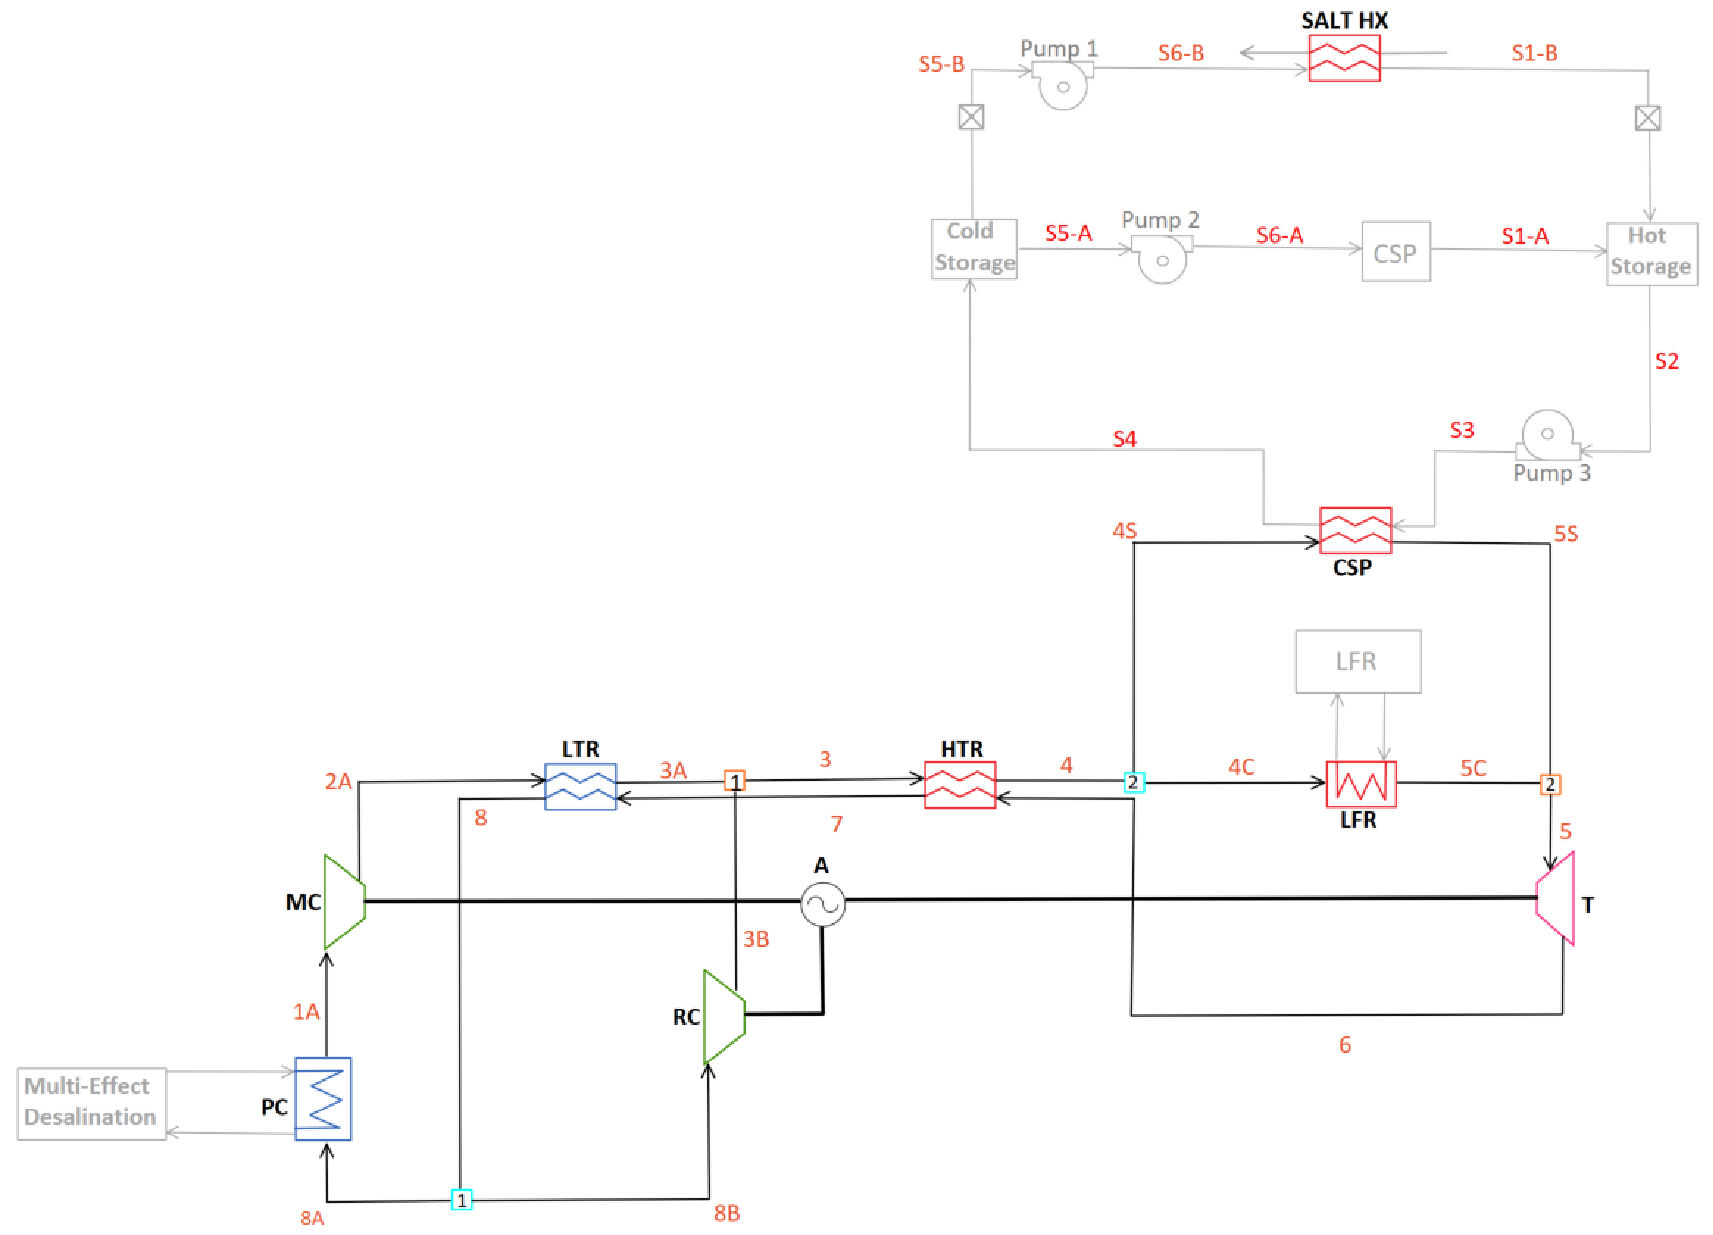
\includegraphics[width=\linewidth]{Definitions/c-1htr1t-on.pdf}
    \caption{Diagram for C-1HTR1T-ON with focus on electricity generation\label{c-1htr1t-on}}
\end{figure}
\begin{paracol}{2}
\linenumbers
\switchcolumn

In this cycle the LFR and CSP are linked due to the parallel orientation. Therefore, three sensitivity studies were done on the C-1HTR1T-ON EES model. The initial two studies had the low LFR temperature constrained to the value of 673.2 K with varied cold CSP TES and maximized cycle efficiency. The two tested values for cold CSP TES with constrained LFR low temperature were 683.2 K and 713.2 K. The desired cold CSP TES temperature of 663.2 K was not possible with the constraint on the LFR low temperature. To obtain the desired cold CSP TES temperature, the constraint was removed droping the temperature of the LFR inlet to 653.2 K. These values are displayed in Table \ref{tab-c-1htr1t-on}.

\begin{specialtable}[H] 
    \caption{Calculated system parameters for non-charging C-1HTR1T-ON cycle configuration with constrained (\textit{C}) and unconstrained (\textit{U}) Lead-Fast Reactor low-end temperature. Temperature of TES cold temperature is also varied.\label{tab-c-1htr1t-on}}
    \begin{tabular}{lcccc}
    \toprule
    \textbf{Definition} & \textbf{Variable} & \textbf{C-1HTR1T-ON}\\
    & & \textit{U} & \textit{C} & \textit{C}\\
    \midrule
    Cold TES Temperature (K)	&	$T_{CS}$	&	Data	&	Data	&	Data	\\
    LFR Inlet Temperature (K)	&	$T_{4C}$	&	Data	&	Data	&	Data	\\
    Cycle Efficiency (\%)	&	$\eta_{cycle}$	&	Data	&	Data	&	Data	\\
    Alternator Power (W)	&	$\dot{W}_{A}$	&	Data	&	Data	&	Data	\\
    PC Heat Transfer	&	$\dot{Q}_{PC}$	&	Data	&	Data	&	Data	\\
    MC Power (W)	&	$\dot{W}_{MC}$	&	Data	&	Data	&	Data	\\
    RC Power (W)	&	$\dot{W}_{RC}$	&	Data	&	Data	&	Data	\\
    Turbine Power (W)	&	$\dot{W}_{T}$	&	Data	&	Data	&	Data	\\
    MC Mass Flow Fraction (-)	&	$y_{1}$	&	Data	&	Data	&	Data	\\
    LFR Mass Flow Fraction (-)	&	$y_{2}$	&	Data	&	Data	&	Data	\\
    LTR UA Value (W/K)	&	$UA_{LTR}$	&	Data	&	Data	&	Data	\\
    LTR Capacitance Ratio (-)	&	$CR_{LTR}$	&	Data	&	Data	&	Data	\\
    LTR Heat Transfer Rate (W)	&	$\dot{Q}_{LTR}$	&	Data	&	Data	&	Data	\\
    LTR Effectiveness (-)	&	$\varepsilon_{LTR}$	&	Data	&	Data	&	Data	\\
    HTR UA Value (W/K)	&	$UA_{HTR}$	&	Data	&	Data	&	Data	\\
    HTR Capacitance Ratio (-)	&	$CR_{HTR}$	&	Data	&	Data	&	Data	\\
    HTR Heat Transfer Rate (W)	&	$\dot{Q}_{HTR}$	&	Data	&	Data	&	Data	\\
    HTR Effectiveness (-)	&	$\varepsilon_{HTR}$	&	Data	&	Data	&	Data	\\
    CSPHX UA Value (W/K)	&	$UA_{CSPHX}$	&	Data	&	Data	&	Data	\\
    CSPHX Capacitance Ratio (-)	&	$CR_{CSPHX}$	&	Data	&	Data	&	Data	\\
    CSPHX Heat Transfer Rate (W)	&	$\dot{Q}_{CSPHX}$	&	Data	&	Data	&	Data	\\
    CSPHX Effectiveness (-)	&	$\varepsilon_{CSPHX}$	&	Data	&	Data	&	Data	\\
    \bottomrule
    \end{tabular}\\
\end{specialtable}

\textbf{Discussion of Results}

\subsubsection{C-2HTR3T-ON} %-----------------------------------------------------

Mixing two different temperature flows before the turbine in a Brayton cycle has a negative effect on cycle efficiency. To quantify the reduction in cycle efficiency, another cycle with no mixing prior to the turbine was desired. This cycle is labeled at C-2HTR3T-ON. This cycle, seen in Figure \ref{c-2htr3t-on}, has two high temperature recuperators and three turbines.

\end{paracol}
\begin{figure}[H]
    \widefigure
    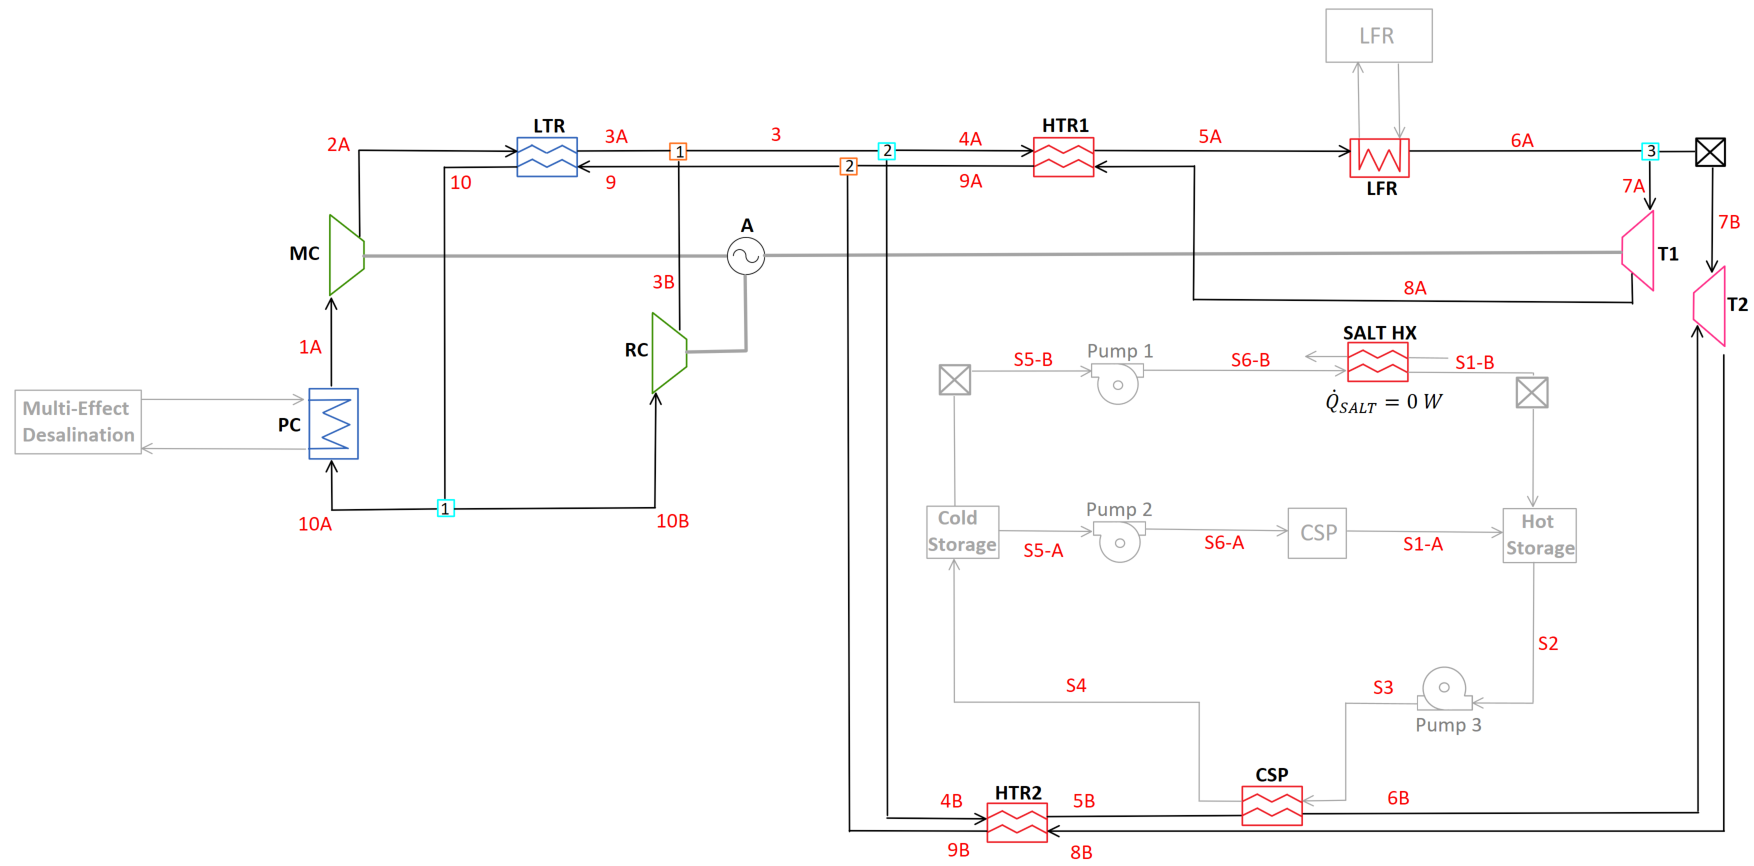
\includegraphics[width=\linewidth]{Definitions/c-2htr3t-on.pdf}
    \caption{Diagram for C-2HTR3T-ON with focus on electricity generation\label{c-2htr3t-on}}
\end{figure}
\begin{paracol}{2}
\linenumbers
\switchcolumn

Three sensitivity studies were done on the C-2HTR3T-ON model. Two with the LFR low temperature constrained and one without this constraint. The two constrained studies had varied cold CSP TES temperature with the lowest temperautre of 663.2 K and highest temperature of 713.2 K. The unconstrained low LFR inlet study was done at a cold CSP TES temperature of 663.2 K. The calculated values from these studies are displayed in Table \ref{tab-c-2htr3t-on}. 

\begin{specialtable}[H]
    \caption{Calculated system parameters for non-charging C-2HTR3T-ON cycle configuration with constrained (\textit{C}) and unconstrained (\textit{U}) Lead-Fast Reactor low-end temperature.\label{tab-c-2htr3t-on}}
    \begin{tabular}{lcccc}
    \toprule
    \textbf{Definition} & \textbf{Variable} & \textbf{C-2HTR3T-ON} &\\
    & & \textit{U} & \textit{C} & \textit{C}\\
    \midrule	
    Cold TES Temperature (K)	&	$T_{CS}$	&	Data	&	Data	&	Data	\\
    LFR Inlet Temperature (K)	&	$T_{5A}$	&	Data	&	Data	&	Data	\\
    Cycle Efficiency (\%)	&	$\eta_{cycle}$	&	Data	&	Data	&	Data	\\
    Alternator Power (W)	&	$\dot{W}_{A}$	&	Data	&	Data	&	Data	\\
    PC Heat Transfer	&	$\dot{Q}_{PC}$	&	Data	&	Data	&	Data	\\
    MC Power (W)	&	$\dot{W}_{MC}$	&	Data	&	Data	&	Data	\\
    RC Power (W)	&	$\dot{W}_{RC}$	&	Data	&	Data	&	Data	\\
    T1 Power (W)	&	$\dot{W}_{T1}$	&	Data	&	Data	&	Data	\\
    T2 Power (W)	&	$\dot{W}_{T2}$	&	Data	&	Data	&	Data	\\
    MC Mass Flow Fraction (-)	&	$y_{1}$	&	Data	&	Data	&	Data	\\
    LFR Mass Flow Fraction (-)	&	$y_{2}$	&	Data	&	Data	&	Data	\\
    LTR UA Value (W/K)	&	$UA_{LTR}$	&	Data	&	Data	&	Data	\\
    LTR Capacitance Ratio (-)	&	$CR_{LTR}$	&	Data	&	Data	&	Data	\\
    LTR Heat Transfer Rate (W)	&	$\dot{Q}_{LTR}$	&	Data	&	Data	&	Data	\\
    LTR Effectiveness (-)	&	$\varepsilon_{LTR}$	&	Data	&	Data	&	Data	\\
    HTR1 UA Value (W/K)	&	$UA_{HTR1}$	&	Data	&	Data	&	Data	\\
    HTR1 Capacitance Ratio (-)	&	$CR_{HTR1}$	&	Data	&	Data	&	Data	\\
    HTR1 Heat Transfer Rate (W)	&	$\dot{Q}_{HTR1}$	&	Data	&	Data	&	Data	\\
    HTR1 Effectiveness (-)	&	$\varepsilon_{HTR1}$	&	Data	&	Data	&	Data	\\
    HTR2 UA Value (W/K)	&	$UA_{HTR2}$	&	Data	&	Data	&	Data	\\
    HTR2 Capacitance Ratio (-)	&	$CR_{HTR2}$	&	Data	&	Data	&	Data	\\
    HTR2 Heat Transfer Rate (W)	&	$\dot{Q}_{HTR2}$	&	Data	&	Data	&	Data	\\
    HTR2 Effectiveness (-)	&	$\varepsilon_{HTR2}$	&	Data	&	Data	&	Data	\\
    CSPHX UA Value (W/K)	&	$UA_{CSPHX}$	&	Data	&	Data	&	Data	\\
    CSPHX Capacitance Ratio (-)	&	$CR_{CSPHX}$	&	Data	&	Data	&	Data	\\
    CSPHX Heat Transfer Rate (W)	&	$\dot{Q}_{CSPHX}$	&	Data	&	Data	&	Data	\\
    CSPHX Effectiveness (-)	&	$\varepsilon_{CSPHX}$	&	Data	&	Data	&	Data	\\
    \bottomrule
    \end{tabular}\\
\end{specialtable}

\textbf{Discussion of Results}

\subsection{Thermal Energy Storage Charging Techniques} %=========================

When the grid demand is not high, the non-charging cycle configurations focus on an energy storage operating mode. Alternator power is set to zero and power from the turbine is solely powering the two compressors. The excess energy from the LFR is thermally stored in the TES for later use instead of generating electricity. Comparison of where thermal energy is drawn from the cycle is done by using the same recompression cycle and configuring the salt heat exchanger in different locations around the turbine. 

\subsubsection{C-LFR-PRE} %-------------------------------------------------------

Flow leaves the turbine with excess thermal energy that was not transformed into mechanical energy. This thermal energy can be used to charge the hot CSP TES. The diagram outlining this process is C-LFR-PRE in Figure \ref{c-lfr-pre}.  

\end{paracol}
\begin{figure}[H]
    \widefigure
    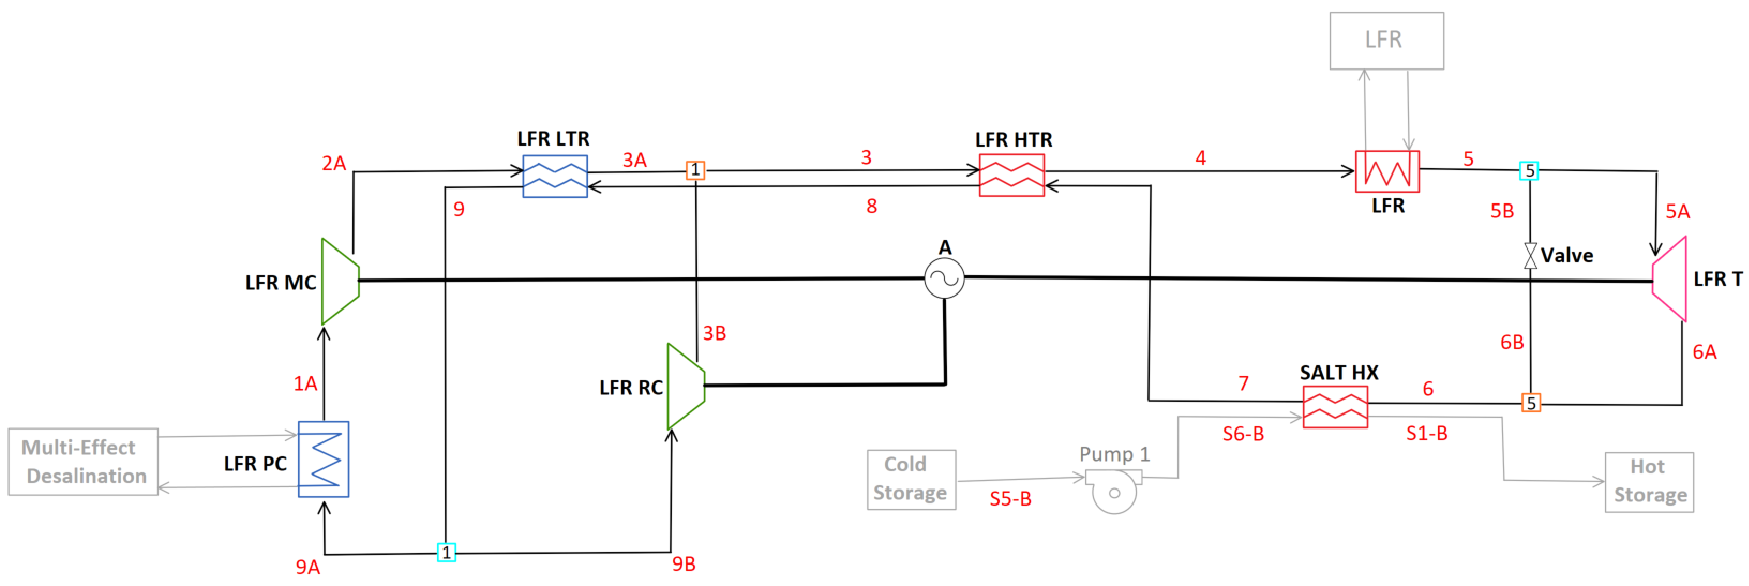
\includegraphics[width=\linewidth]{Definitions/c-lfr-pre.pdf}
    \caption{Diagram for C-LFR-PRE thermal energy storage charging orientation\label{c-lfr-pre}}
\end{figure}
\begin{paracol}{2}
\linenumbers
\switchcolumn

Problems arise with this salt charging configuration. The primary issue is that the temperature out of the turbine is not high enough to charge the hot CSP TES to the required value of 833.2 K. To raise the temperature, some of the high temperature flow before the turbine is redirected through a valve and combined after the turbine. This combination of different temperature flows has a large impact on heat storage efficiency. The calculations from this TES charging technique are shown in Table \ref{tab-c-lfr-pre}.

\begin{specialtable}[H]
    \caption{Calculated system parameters for salt charging C-LFR-PRE cycle configuration with TES cold storage set to 663.2 K.\label{tab-c-lfr-pre}}
    \begin{tabular}{lcc}
    \toprule
    \textbf{Definition} & \textbf{Variable} & \textbf{C-LFR-PRE}\\
    & & \textit{C}\\
    \midrule	
    Cold TES Temperature (K)	&	$T_{CS}$	&	Data	\\
    LFR Inlet Temperature (K)	&	$T_{4}$	&	Data	\\
    Heat Storage Efficiency (\%)	&	$\eta_{heatstorage}$	&	Data	\\
    Alternator Power (W)	&	$\dot{W}_{A}$	&	Data	\\
    PC Heat Transfer	&	$\dot{Q}_{PC}$	&	Data	\\
    MC Power (W)	&	$\dot{W}_{MC}$	&	Data	\\
    RC Power (W)	&	$\dot{W}_{RC}$	&	Data	\\
    Turbine Power (W)	&	$\dot{W}_{T}$	&	Data	\\
    MC Mass Flow Fraction (-)	&	$y_{1}$	&	Data	\\
    Valve Mass Flow Fraction (-)	&	$y_{5}$	&	Data	\\
    LTR UA Value (W/K)	&	$UA_{LTR}$	&	Data	\\
    LTR Capacitance Ratio (-)	&	$CR_{LTR}$	&	Data	\\
    LTR Heat Transfer Rate (W)	&	$\dot{Q}_{LTR}$	&	Data	\\
    LTR Effectiveness (-)	&	$\varepsilon_{LTR}$	&	Data	\\
    HTR UA Value (W/K)	&	$UA_{HTR}$	&	Data	\\
    HTR Capacitance Ratio (-)	&	$CR_{HTR}$	&	Data	\\
    HTR Heat Transfer Rate (W)	&	$\dot{Q}_{HTR}$	&	Data	\\
    HTR Effectiveness (-)	&	$\varepsilon_{HTR}$	&	Data	\\
    CSPHX UA Value (W/K)	&	$UA_{CSPHX}$	&	Data	\\
    CSPHX Capacitance Ratio (-)	&	$CR_{CSPHX}$	&	Data	\\
    CSPHX Heat Transfer Rate (W)	&	$\dot{Q}_{CSPHX}$	&	Data	\\
    CSPHX Effectiveness (-)	&	$\varepsilon_{CSPHX}$	&	Data	\\
    \bottomrule
    \end{tabular}\\
\end{specialtable}

\textbf{Discussion of Results}

\subsubsection{C-LFR-POST} %------------------------------------------------------

Moving the heat extraction prior to the turbine was qualitatively analyzed in C-LFR-POST. This diagram is seen in Figure \ref{c-lfr-post}.

\end{paracol}
\begin{figure}[H]
    \widefigure
    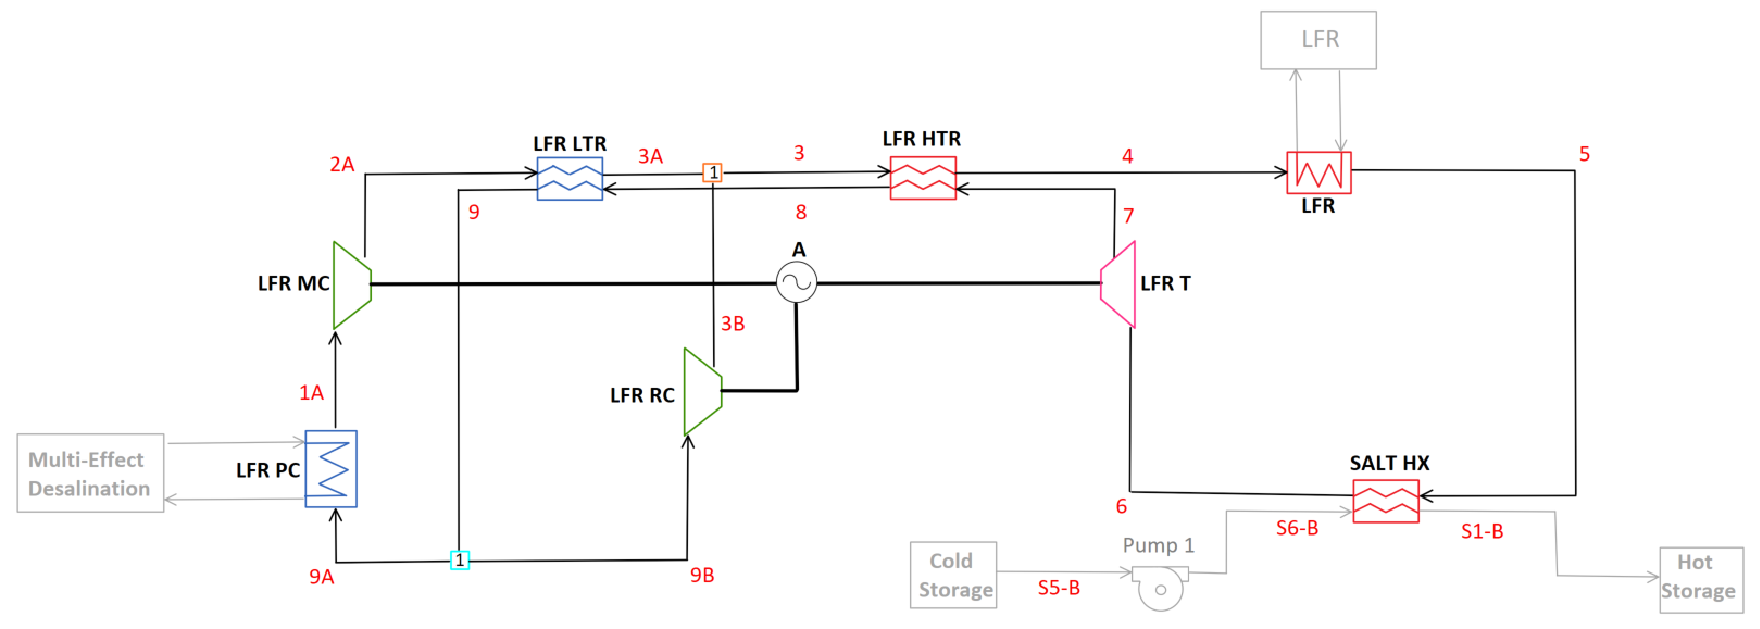
\includegraphics[width=\linewidth]{Definitions/c-lfr-post.pdf}
    \caption{Diagram for C-LFR-POST thermal energy storage charging orientation\label{c-lfr-post}}
\end{figure}
\begin{paracol}{2}
\linenumbers
\switchcolumn

This TES charging cycle was extracting heat before the turbine and therefore would have a large negative effect on the amount of work that the turbine could produce. The turbine needs to offset the requirements of both compressors and this would require the inlet temperature to be high. The amount of energy that could be extracted before the turbine would be small and therefore the heat storage efficiency would be small. There was no quantitative study done on this diagram because it theoreticaly would be non-viable. 

\subsubsection{C-LFR-PAR} %-------------------------------------------------------

The requirement of the turbine and hot CSP TES temperature could be accomplished by splitting the flow before the turbine. The flow through the salt heat exchanger would therefore be seperate from the turbine. After the salt heat exchanger a valve would need to reduce the pressure, this TES charging cycle is C-LFR-PAR shown in Figure \ref{c-lfr-par}.

\end{paracol}
\begin{figure}[H]
    \widefigure
    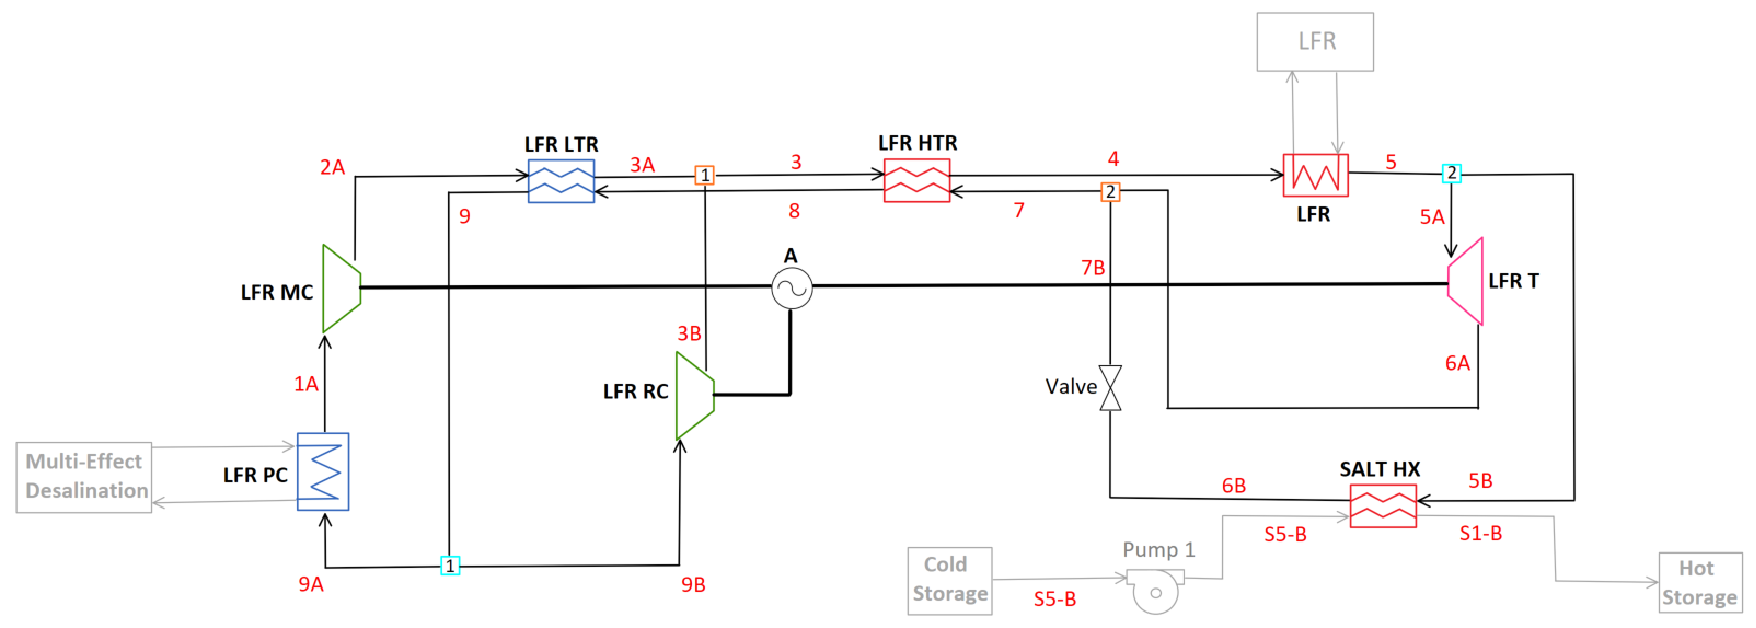
\includegraphics[width=\linewidth]{Definitions/c-lfr-par.pdf}
    \caption{Diagram for C-LFR-PAR thermal energy storage charging orientation\label{c-lfr-par}}
\end{figure}
\begin{paracol}{2}
\linenumbers
\switchcolumn

This cycle had two sensitivity studies done with varying cold CSP TES. The low temperature study was done at 663.2 K and the high temperature study was done at 713.2 K. The results from this study are displayed in Table \ref{tab-c-lfr-par}.

\begin{specialtable}[H]
    \caption{Calculated system parameters for salt charging C-LFR-PAR cycle configuration with TES cold storage varied and LFR low temperature set to 673.2 K.\label{tab-c-lfr-par}}
    \begin{tabular}{lccc}
    \toprule
    \textbf{Definition} & \textbf{Variable} & \textbf{C-2HTR3T-ON} & \\
    & & \textit{C} & \textit{C}\\
    \midrule	
    Cold TES Temperature (K)	&	$T_{CS}$	&	Data	&	Data	\\
    LFR Inlet Temperature (K)	&	$T_{4}$	&	Data	&	Data	\\
    Heat Storage Efficiency (\%)	&	$\eta_{heatstorage}$	&	Data	&	Data	\\
    Alternator Power (W)	&	$\dot{W}_{A}$	&	Data	&	Data	\\
    PC Heat Transfer	&	$\dot{Q}_{PC}$	&	Data	&	Data	\\
    MC Power (W)	&	$\dot{W}_{MC}$	&	Data	&	Data	\\
    RC Power (W)	&	$\dot{W}_{RC}$	&	Data	&	Data	\\
    Turbine Power (W)	&	$\dot{W}_{T}$	&	Data	&	Data	\\
    MC Mass Flow Fraction (-)	&	$y_{1}$	&	Data	&	Data	\\
    SALT HX Mass Flow Fraction (-)	&	$y_{2}$	&	Data	&	Data	\\
    LTR UA Value (W/K)	&	$UA_{LTR}$	&	Data	&	Data	\\
    LTR Capacitance Ratio (-)	&	$CR_{LTR}$	&	Data	&	Data	\\
    LTR Heat Transfer Rate (W)	&	$\dot{Q}_{LTR}$	&	Data	&	Data	\\
    LTR Effectiveness (-)	&	$\varepsilon_{LTR}$	&	Data	&	Data	\\
    HTR UA Value (W/K)	&	$UA_{HTR}$	&	Data	&	Data	\\
    HTR Capacitance Ratio (-)	&	$CR_{HTR}$	&	Data	&	Data	\\
    HTR Heat Transfer Rate (W)	&	$\dot{Q}_{HTR}$	&	Data	&	Data	\\
    HTR Effectiveness (-)	&	$\varepsilon_{HTR}$	&	Data	&	Data	\\
    CSPHX UA Value (W/K)	&	$UA_{CSPHX}$	&	Data	&	Data	\\
    CSPHX Capacitance Ratio (-)	&	$CR_{CSPHX}$	&	Data	&	Data	\\
    CSPHX Heat Transfer Rate (W)	&	$\dot{Q}_{CSPHX}$	&	Data	&	Data	\\
    CSPHX Effectiveness (-)	&	$\varepsilon_{CSPHX}$	&	Data	&	Data	\\
    CSPHX Approach Temperature (K)	&	$\delta_{CSPHX}$	&	Data	&	Data	\\
    
    \bottomrule
    \end{tabular}\\
\end{specialtable}

Changing the temperature of the cold CSP TES had little effect on the heat storage efficiency. The CSP salt mass flow rate and approach temperature of the SALT HX would adjust according to the temperature difference in the TES and keep the efficiency constant.

\subsubsection{C-LFR-CIRC} %------------------------------------------------------

The full diagram for C-LFR-CIRC is shown in Figure \ref{c-lfr-circ}.

\end{paracol}
\begin{figure}[H]
    \widefigure
    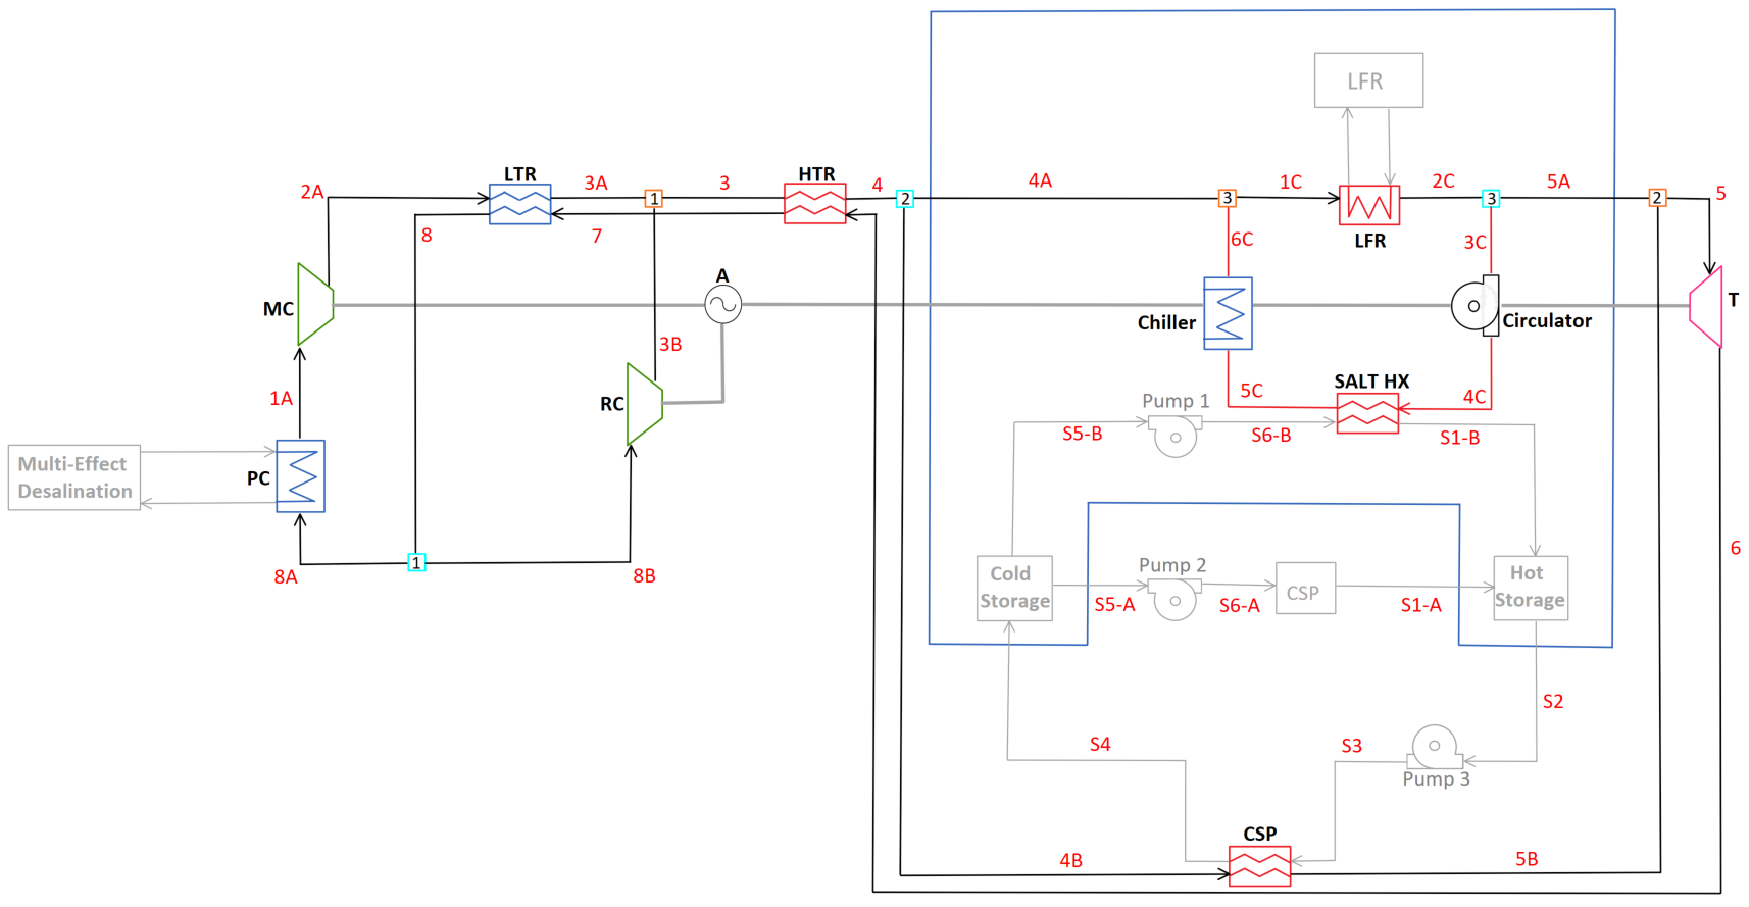
\includegraphics[width=\linewidth]{Definitions/c-lfr-circ.pdf}
    \caption{Full diagram for C-LFR-CIRC thermal energy storage charging orientation\label{c-lfr-circ}}
\end{figure}
\begin{paracol}{2}
\linenumbers
\switchcolumn

The charging subsection of this diagram is composed of a circulation cycle that has heat inputed through the LFR heat exchanger. This subsection is seen in Figure \ref{c-lfr-circ-sub}.


\end{paracol}
\begin{figure}[H]
    \widefigure
    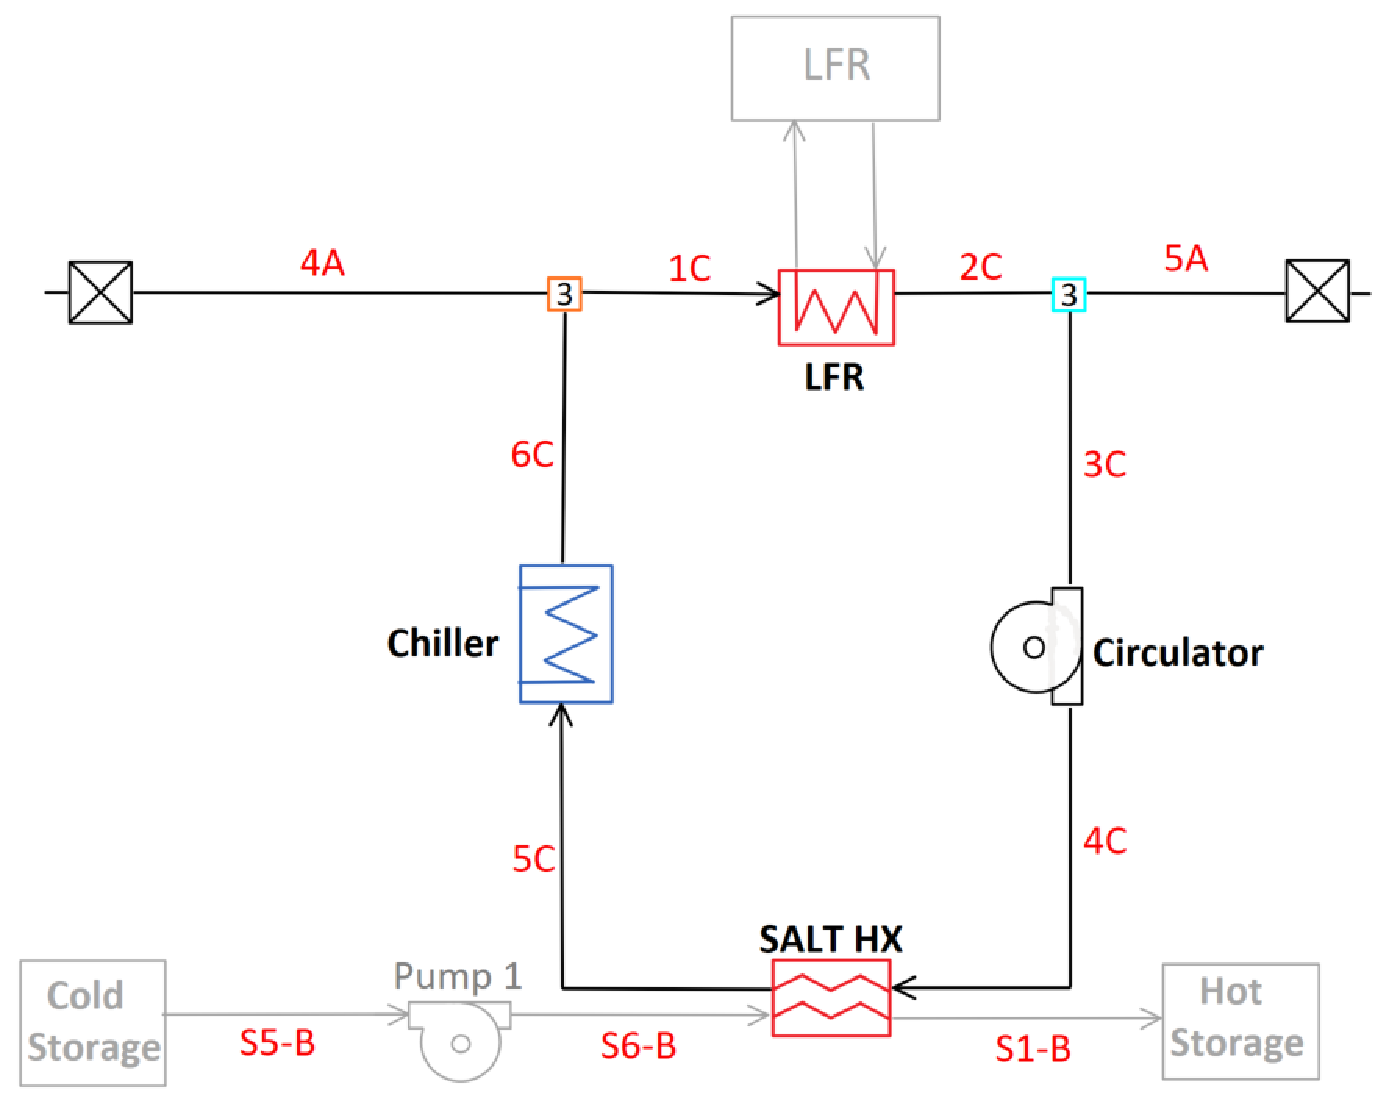
\includegraphics[width=10 cm]{Definitions/c-lfr-circ-sub.pdf}
    \caption{Diagram for C-LFR-CIRC subcycle thermal energy storage charging orientation\label{c-lfr-circ-sub}}
\end{figure}
\begin{paracol}{2}
\linenumbers
\switchcolumn

The flow then continues through a circulator which has neglegible pressure rise. A heat exchanger then extracts heat from the flow, transfering into the hot TES for later use. Excess heat that is not extracted is then dumped into a reservior through the chiller to bring the temperature of the flow down to LFR cool side operating temperature of 673.2 K. Three different temperatures; 663.2 K, 683.2 K, and 713.2 K, are compared in Table \ref{tab-c-lfr-circ} to show cold thermal energy storage's affect on heat storage efficiency.\\

\begin{specialtable}[H]
    \caption{Calculated system parameters for charging C-LFR-CIRC subcycle configuration with constrained Lead-Fast Reactor low-end temperature.\label{tab-c-lfr-circ}}
    \begin{tabular}{lcccc}
    \toprule
    \textbf{Definition} & \textbf{Variable} & \textbf{C-LFR-CIRC} &\\
    \midrule	
    Cold TES Temperature (K)	&	$T_{CS}$	&	Data	&	Data	&	Data	\\
    LFR Inlet Temperature (K)	&	$T_{1C}$	&	Data	&	Data	&	Data	\\
    Heat Storage Efficiency (\%)	&	$\eta_{heatstorage}$	&	Data	&	Data	&	Data	\\
    Chiller Heat Transfer (W)	&	$\dot{Q}_{chill}$	&	Data	&	Data	&	Data	\\
    CSPHX UA Value (W/K)	&	$UA_{CSPHX}$	&	Data	&	Data	&	Data	\\
    CSPHX Capacitance Ratio (-)	&	$CR_{CSPHX}$	&	Data	&	Data	&	Data	\\
    CSPHX Heat Transfer Rate (W)	&	$\dot{Q}_{CSPHX}$	&	Data	&	Data	&	Data	\\
    CSPHX Effectiveness (-)	&	$\varepsilon_{CSPHX}$	&	Data	&	Data	&	Data	\\
    \bottomrule
    \end{tabular}\\
\end{specialtable}



%%%%%%%%%%%%%%%%%%%%%%%%%%%%%%%%%%%%%%%%%%
\section{Discussion}

Authors should discuss the results and how they can be interpreted from the perspective of previous studies and of the working hypotheses. The findings and their implications should be discussed in the broadest context possible. Future research directions may also be highlighted.

%%%%%%%%%%%%%%%%%%%%%%%%%%%%%%%%%%%%%%%%%%
\section{Conclusions}

This section is not mandatory, but can be added to the manuscript if the discussion is unusually long or complex.

%%%%%%%%%%%%%%%%%%%%%%%%%%%%%%%%%%%%%%%%%%
\section{how to use}

\subsection{Subsection}
Citing a journal paper \cite{wagner2017optimization} . Now citing a book reference \cite{blair2005sam} or other reference types \cite{hirsch2011standardization}. \cite{nellis_klein_2008}
\subsubsection{Subsubsection}

Bulleted lists look like this:
\begin{itemize}
\item	First bullet;
\item	Second bullet;
\item	Third bullet.
\end{itemize}

Numbered lists can be added as follows:
\begin{enumerate}
\item	First item; 
\item	Second item;
\item	Third item.
\end{enumerate}

The text continues here. 

\subsection{Figures, Tables and Schemes}

All figures and tables should be cited in the main text as Figure~\ref{fig1}, Table~\ref{tab1}, etc.

\begin{figure}[H]

\includegraphics[width=10.5 cm]{Definitions/logo-mdpi}
\caption{This is a figure. Schemes follow the same formatting. If there are multiple panels, they should be listed as: (\textbf{a}) Description of what is contained in the first panel. (\textbf{b}) Description of what is contained in the second panel. Figures should be placed in the main text near to the first time they are cited. A caption on a single line should be centered.\label{fig1}}
\end{figure}   

% The MDPI table float is called specialtable
\begin{specialtable}[H] 
\caption{This is a table caption. Tables should be placed in the main text near to the first time they are~cited.\label{tab1}}
%%% \tablesize{} %% You can specify the fontsize here, e.g., \tablesize{\footnotesize}. If commented out \small will be used.
\begin{tabular}{ccc}
\toprule
\textbf{Title 1}	& \textbf{Title 2}	& \textbf{Title 3}\\
\midrule
Entry 1		& Data			& Data\\
Entry 2		& Data			& Data\\
\bottomrule
\end{tabular}
\end{specialtable}

%\begin{listing}[H]
%\caption{Title of the listing}
%\rule{\columnwidth}{1pt}
%\raggedright Text of the listing. In font size footnotesize, small, or normalsize. Preferred format: left aligned and single spaced. Preferred border format: top border line and bottom border line.
%\rule{\columnwidth}{1pt}
%\end{listing}

Text.

Text.

\subsection{Formatting of Mathematical Components}

This is the example 1 of equation:
\begin{equation}
a = 1,
\end{equation}
the text following an equation need not be a new paragraph. Please punctuate equations as regular text.
%% If the documentclass option "submit" is chosen, please insert a blank line before and after any math environment (equation and eqnarray environments). This ensures correct linenumbering. The blank line should be removed when the documentclass option is changed to "accept" because the text following an equation should not be a new paragraph.

This is the example 2 of equation:
\end{paracol}
\nointerlineskip
\begin{eqnarray}
a &=& b + c + d + e + f + g + h + i + j + k + l\nonumber \\
 &+& m + n + o + p + q + r + s + t + u + v + w + x + y + z %\nonumber
\end{eqnarray}

% Example of a figure that spans the whole page width (the commands \widefigure and \begin{paracol}{2}, \linenumbers, and\switchcolumn need to be present). The same concept works for tables, too.
%\begin{figure}[H]	
%\widefigure
%
\includegraphics[width=15 cm]{Definitions/logo-mdpi}
%\caption{This is a wide figure.\label{fig2}}
%\end{figure} 





\begin{paracol}{2}
\linenumbers
\switchcolumn
Please punctuate equations as regular text. Theorem-type environments (including propositions, lemmas, corollaries etc.) can be formatted as follows:
%% Example of a theorem:
\begin{Theorem}
Example text of a theorem.
\end{Theorem}

The text continues here. Proofs must be formatted as follows:

%% Example of a proof:
\begin{proof}[Proof of Theorem 1]
Text of the proof. Note that the phrase ``of Theorem 1'' is optional if it is clear which theorem is being referred to.
\end{proof}
The text continues here.

\end{paracol}
